\chapter{Geometrie Non Euclidee}

La teoria che studieremo è una \textit{teoria geometrica}:

\textbf{I 5 postulati di Euclide:}
\begin{enumerate}
    \item Per due qualsiasi punti $A$ e $B$, esiste esattamente una retta che li attraversa.
    \item Una retta può essere prolungata indefinitamente in entrambe le direzioni.
    \item Dato un punto $O$ ed un raggio $R$, esiste esattamente un cerchio con centro in $O$ e raggio $R$.
    \item Tutti gli angoli retti sono congruenti.
    \item Data una retta r ed un punto P fuori da essa, per
    il punto P passa una ed una sola retta parallela ad r (possiamo dare al termine parallelo il significato di \textit{che incontra r solo all'infinito}, in un punto improprio).
\end{enumerate}

Il quinto postulato è più complesso degli altri; i tentativi di dimostrare tale postulato a partire dagli altri postulati, considerati più evidenti, non hanno permesso di arrivare a questo, ma hanno portato, nell'800, alla nascita delle geometrie non-Euclidee (Gauss, Bolyai, Lobachevski, Klein).

\begin{center}
\begin{tikzpicture}[scale=1.0]
    % Draw a dashed line at the top
    \draw[dashed] (-3,1) -- (3,1);
    % Create point P at the center of the dashed line
    \fill (0,1) circle (1pt) node[above] {$P$};
    % Draw the line r at the bottom
    \draw (-3,0) -- (3,0);
    % Place the label r at the left end of the line
    \node at (-2.9,0) [left, above] {$r$};
\end{tikzpicture}
\end{center}

Il quinto postulato si è rivelato indipendente dagli altri enunciati di Euclide, poiché è stato possibile formulare geometrie piane (in 2 dimensioni) in cui valgono tutti gli altri postulati, mentre il concetto di parallelismo assume un significato diverso:

\begin{enumerate}
    \item Non esiste alcuna retta parallela a $R$ passante per $P$ \,\quad $\rightarrow$ \textbf{Geometrie ellittiche piane} $[S^2]$
    \item Esistono due o più rette parallele a $R$ passanti per $P$ \quad $\rightarrow$ \textbf{Geometrie iperboliche piane} $[H^2]$
\end{enumerate}

\begin{figure}[H]
    \centering
    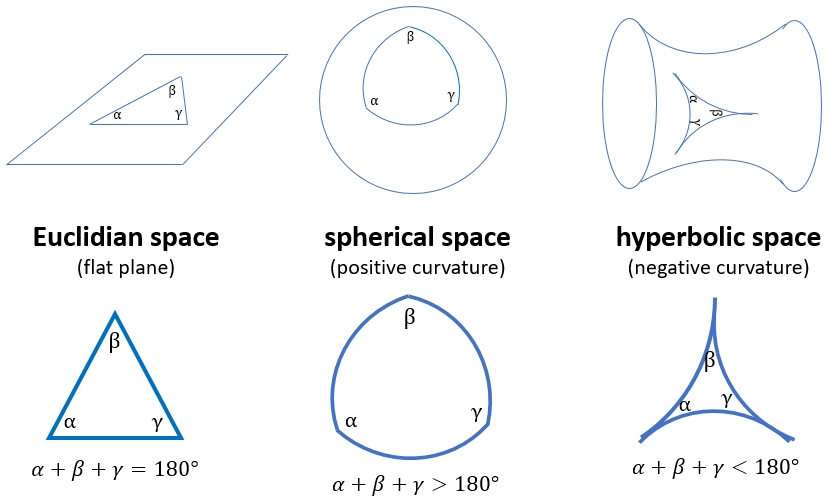
\includegraphics[width=0.6\textwidth]{assets/geometries.png}
    \caption{Geometrie ellittiche e iperboliche}
\end{figure}

\subsection{Geometria Ellittica}

La \textbf{geometria ellittica piana} è una forma di geometria non euclidea che rifiuta il quinto postulato di Euclide, il quale in geometria euclidea garantisce l'esistenza di una sola retta parallela passante per un dato punto. In geometria ellittica, non esistono rette parallele; invece, ogni coppia di rette si interseca eventualmente.

Un classico esempio è la geometria sferica, in cui possiamo definire come "\bfit{punto}" la coppia di punti diametralmente opposti $(P, P')$, e come "\bfit{retta}" un cerchio massimo passante per $P$ e $P'$. Si può dimostrare che per due punti $(P, P')$ e $(Q, Q')$ passa esattamente una retta $r$. Inoltre, per un punto $(T, T')$ esterno ad $r$ non passa alcuna retta parallela ad $r$, poiché tutte le rette passanti per $(T, T')$ intersecano $r$ in almeno un punto.

Con la geometria analitica, Descartes ha mostrato che, identificando i punti con coppie di numeri reali e definendo la distanza tra due punti $(x_1, y_1)$ e $(x_2, y_2)$ come $d = \sqrt{(x_2 - x_1)^2 + (y_2 - y_1)^2}$, tutti i postulati di Euclide si riducono a teoremi sui numeri reali.

Definito sulla sfera un triangolo con i lati formati da archi di cerchi massimi, la somma degli angoli $\alpha + \beta + \gamma$ è sempre $> \pi$. L'area $S$ di tale triangolo, se la sfera ha raggio $R$, si può esprimere come $S = R^2(\alpha + \beta + \gamma - \pi)$. Quando $S \to 0$ (mantenendo $R$ fisso), si osserva che $(\alpha + \beta + \gamma) \to \pi$. Questo significa che se il triangolo sferico è molto più piccolo del raggio $R$, la sua differenza da un triangolo piano tende a scomparire, avvicinandosi alla geometria euclidea.

\begin{figure}[H]
    \centering
    \begin{minipage}{0.3\textwidth}
        \centering
        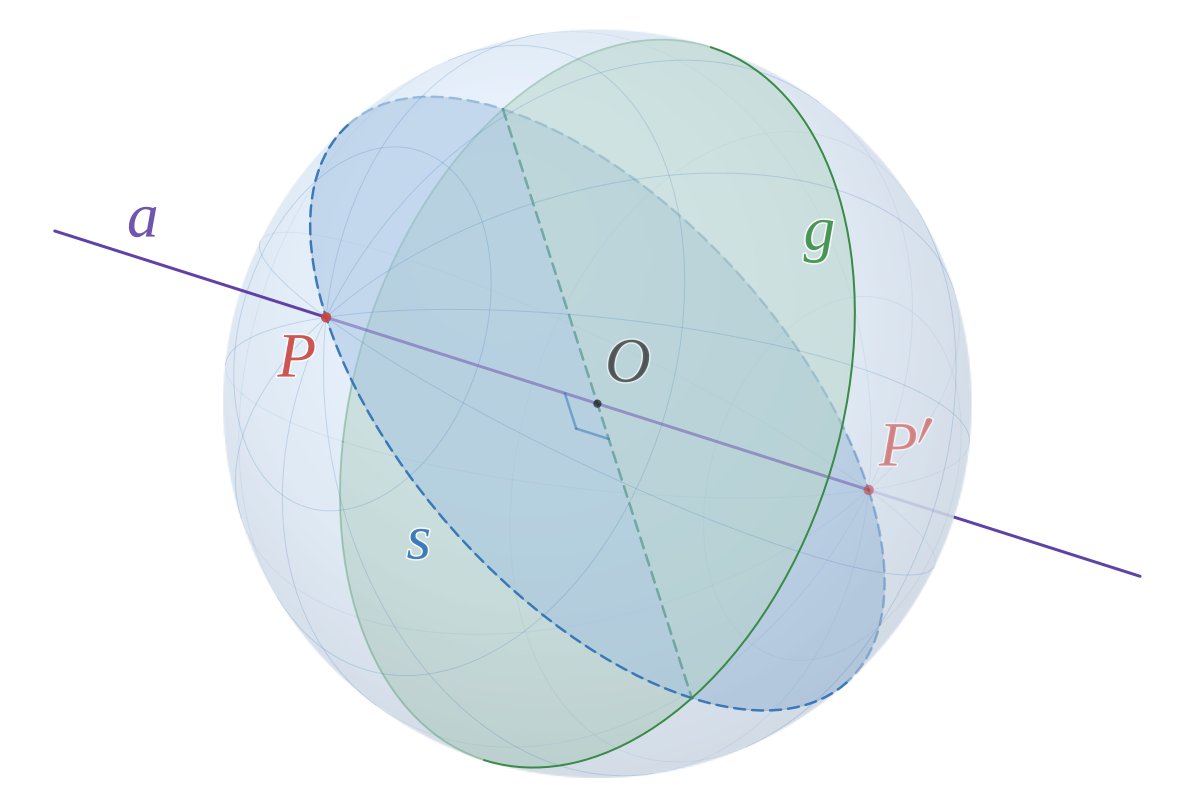
\includegraphics[width=0.85\textwidth]{assets/spherical_geometry.png}
        \caption{Geometria sferica}
    \end{minipage} \hspace{1cm}
    \begin{minipage}{0.3\textwidth}
        \centering
        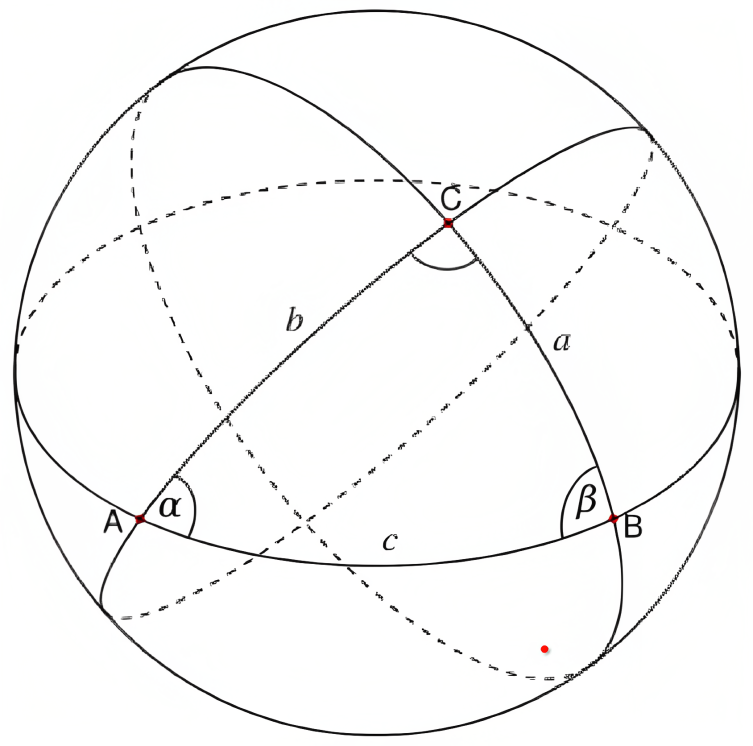
\includegraphics[width=0.82\textwidth]{assets/spherical_triangle.png}
        \caption{Triangolo sferico}
    \end{minipage}
\end{figure}

\vspace{-1em}

In questo contesto, i triangoli, noti come triangoli sferici, mostrano una proprietà intrigante: la somma dei loro angoli interni supera i 180° ($\alpha + \beta + \gamma > \pi$), un fenomeno noto come eccesso sferico, con l'eccesso proporzionale all'area del triangolo.
\vspace{0.2em}
$$
S = R^2(\alpha + \beta + \gamma - \pi) \quad \text{dove per} \quad R \to \infty \quad \text{si ha} \quad \dfrac S{R^2} \to 0 \quad \text{e} \quad \alpha + \beta + \gamma \to \pi
$$
Per costruire un modello della geometria ellittica piana siamo ricorsi all'uso di una sfera (superficie bidimensionale, indicata con $S^2$) immersa (\textit{embedded}) in uno spazio euclideo tridimensionale $E^3$. 

Notiamo che per rappresentare il 5° postulato abbiamo dovuto ricorrere ad una superficie \textit{curva}, cioè la sfera. Questa curvatura deve essere inoltre costante in tutto il piano perché gli altri postulati descrivono lo spazio come omogeneo, e se la curvatura variasse questa proprietà verrebbe meno.

Questo ci porta a comprendere che le diverse geometrie non euclidee possono essere caratterizzate matematicamente attraverso diverse definizioni di distanza. La curvatura dello spazio diventa quindi un elemento fondamentale per distinguere tra i vari tipi di geometrie:
\begin{itemize}
    \item Curvatura zero → geometria euclidea
    \item Curvatura positiva costante → geometria ellittica
    \item Curvatura negativa costante → geometria iperbolica
\end{itemize}

\subsection{Geometria Iperbolica}

La geometria iperbolica piana è una geometria non euclidea in cui il quinto postulato di Euclide non vale, ammettendo più parallele a una retta data. I triangoli iperbolici hanno somma degli angoli inferiore a 180°, con “difetto” proporzionale all’area. Il piano iperbolico non può essere immerso interamente in uno spazio euclideo 3D, ma esistono modelli come il \emph{cerchio di Klein} (1870), in cui i punti sono all’interno di una circonferenza unitaria e le rette ne sono le corde. Da un punto $P$ passano due parallele a una retta data, e ne esistono infinite che non la intersecano.

\begin{figure}[H]
    \centering
    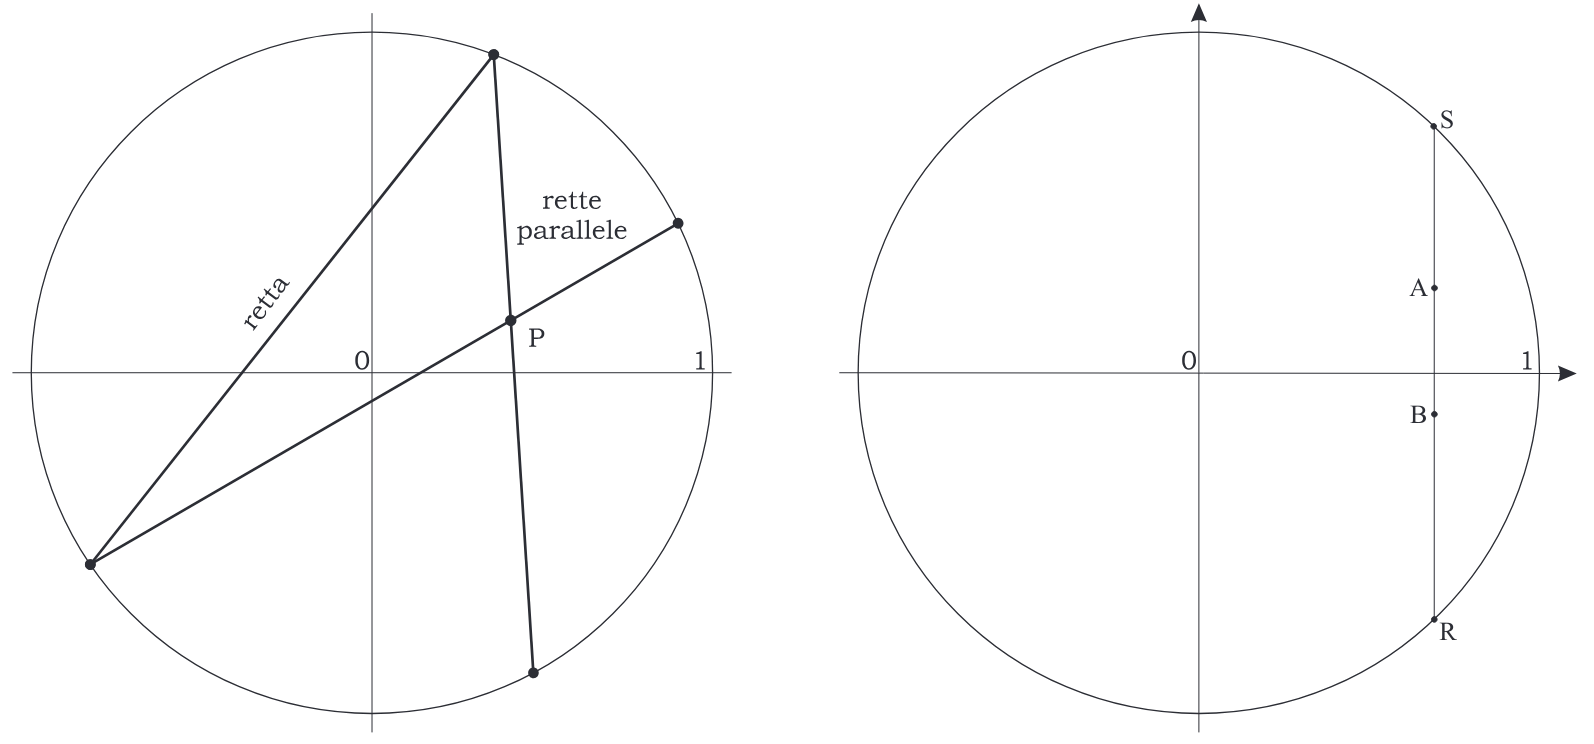
\includegraphics[width=0.75\textwidth]{assets/hyperbolic_geometry.png}
    \caption{Geometria iperbolica}
\end{figure}

\vspace{-1em}

La distanza tra due punti $A$ e $B$ è
$$
d(A,B) = \frac12 \log \!\Bigl(\frac{RA\cdot SB}{RB\cdot SA}\Bigr),
$$
che diverge se uno dei punti tende al bordo. Una rappresentazione parziale di $H^2$ in uno spazio euclideo 3-D $E^3$ è la cosiddetta \bfit{pseudosfera}, una superficie a curvatura negativa costante, in contrasto con la sfera a curvatura positiva.

\section{Curva piana}

Si può parametrizzare una curva piana nel modo seguente: $\bar x(t) = (x_1(t), x_2(t))$, dove $t$ è un parametro, non necessariamente il tempo; il vettore tangente (velocità) è ${d\bar x}/{dt}$. Possiamo definire l'ascissa curvilinea $s(t)$:
$$
O \equiv \bar x(t = 0) \quad P \equiv \bar x(t) \quad ds = |d\bar x| = |\dfrac {d\bar x}{dt}| dt \quad \to \quad s(t) = \int_0^t |d\bar x| = \int_0^t |\dfrac {d\bar x}{dt}| dt
$$

\vspace{-1em}

\begin{figure}[H]
    \centering
    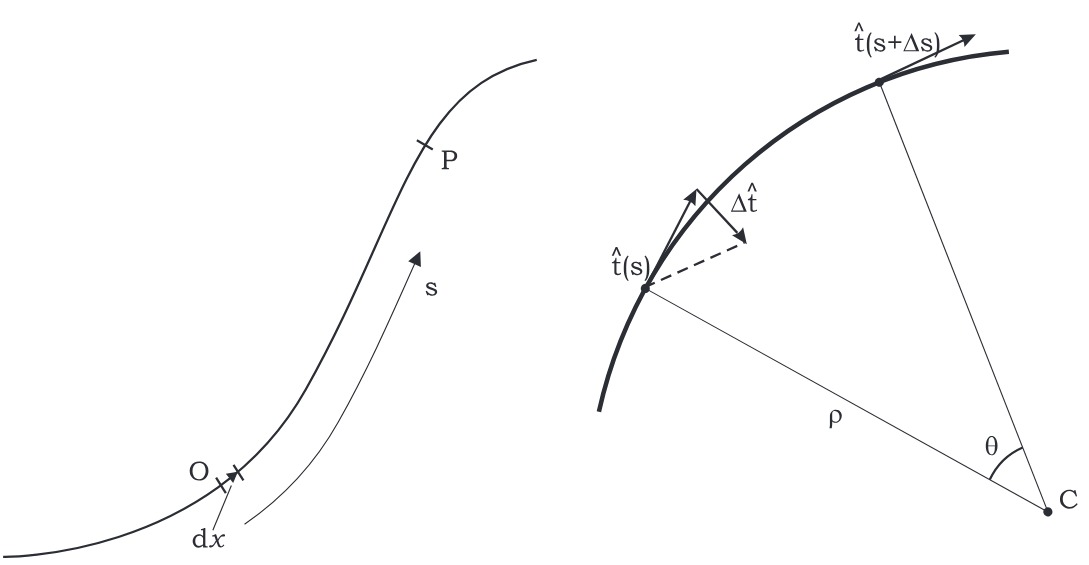
\includegraphics[width=0.6\textwidth]{assets/curve.png}
    \caption{Ascissa curvilinea}
\end{figure}

Applicando la trasformata $t \to s$ notiamo che $\tfrac{d\bar x}{ds} = \dot {\bar x}(s)$ ha modulo 1: è il \textbf{versore tangente} $\hat t(s)$.

Poichè $|\dot {\bar x}(s)| = |\hat t(s)| = 1$, abbiamo $\hat t \cdot {\hat t} = 1$ e, derivando, segue che $2 \hat t \cdot \dot {\hat t} = 0$, ovvero $\hat t \perp \dot {\hat t}$.

$$\boxed{\text{\textbf{Nota}}: \dot {\hat t} \text { non è un versore!}}$$

Separiamo la derivata di $\hat{t}(s)$ in modulo e direzione. Definiamo
$
\kappa(s) \;=\; \bigl|\dot{\hat{t}}(s)\bigr|
\ \ \text{e}\ \
\hat{n}(s) \;=\; \frac{\dot{\hat{t}}(s)}{\bigl|\dot{\hat{t}}(s)\bigr|}
$,
così che
$$
\dot{\hat{t}}(s) \;=\; \kappa(s)\,\hat{n}(s).
$$
Geometricamente, $\kappa$ è la \textbf{curvatura} e $\hat{n}$ il \textbf{versore normale}.

Osserviamo che, se una curva è approssimabile con un arco di cerchio di raggio $\rho$, allora
$$
|\Delta \hat{t}|
\;=\;
2\,|\hat{t}|\sin\!\Bigl(\frac{\Delta \theta}{2}\Bigr)
\;\sim\;
\Delta \theta
\quad\text{e}\quad
\Delta s
\;\simeq\;
\rho\,\Delta \theta.
\quad\text{Da cui}\quad
\left|\frac{\Delta \hat{t}}{\Delta s}\right|
\;\simeq\;
\frac{1}{\rho}.
$$
Nel limite infinitesimo, ciò si traduce in:
$$
\frac{d\hat{t}}{ds}
\;=\;
\kappa\,\hat{n}
\;=\;
\frac{1}{\rho}\,\hat{n}
\quad\Longrightarrow\quad
\begin{cases}
    \kappa\;:\;\text{curvatura},\\
    \rho\;:\;\text{raggio di curvatura}.
\end{cases}
$$
Misurando l’angolo $\theta$ da un riferimento fisso (ad esempio, rispetto all’asse $x$), si ottiene

$$
\Delta s
\;=\;
\rho\,\Delta \theta
\;=\;
\frac{\Delta \theta}{\kappa}
\quad\;\to\;\quad
\kappa
\;=\;
\biggl|\frac{d\theta}{ds}\biggr|.
$$

Finora $\kappa$ è stata definita come grandezza positiva. In corrispondenza di un flesso, ciò comporta però una discontinuità nella direzione di $\hat{n}$. Per ovviare a questo, fissata la parametrizzazione della curva tramite $s$, definiamo $\hat{n}$ come la rotazione di $\hat{t}$ di 90° in senso positivo (coerente con il riferimento $O,x_1,x_2$). Allora $\dot{\hat{t}}$ rimane ortogonale a $\hat{t}$, e possiamo scrivere ancora

\vspace{-1em}

$$\dot{\hat{t}}(s)=\kappa\,\hat{n},$$
ma lasciando che $\kappa$ possa anche assumere valori negativi. In tal modo, in un flesso $\hat{n}$ non cambia, mentre cambia il segno di $\kappa$, permettendo di distinguere se la curvatura si “piega” a sinistra o a destra rispetto alla tangente:
$$
\quad
\phantom{(\text{senza valore assoluto}).}
\kappa
\;=\;
\frac{d\theta}{ds}
\quad
(\text{senza valore assoluto}).
$$

\vspace{-1em}
\begin{figure}[H]
    \centering
    \begin{minipage}{0.3\textwidth}
        \centering
        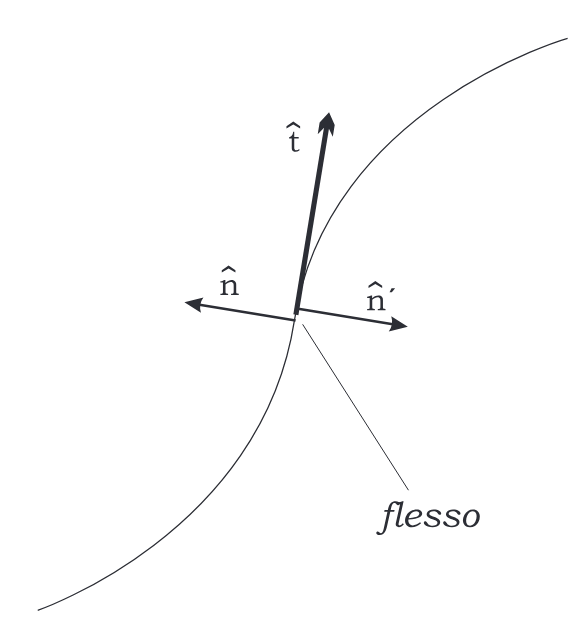
\includegraphics[width=0.95\textwidth]{assets/flesso.png}
    \end{minipage}%
    \hspace{10pt}
    \begin{minipage}{0.65\textwidth}
        \centering
        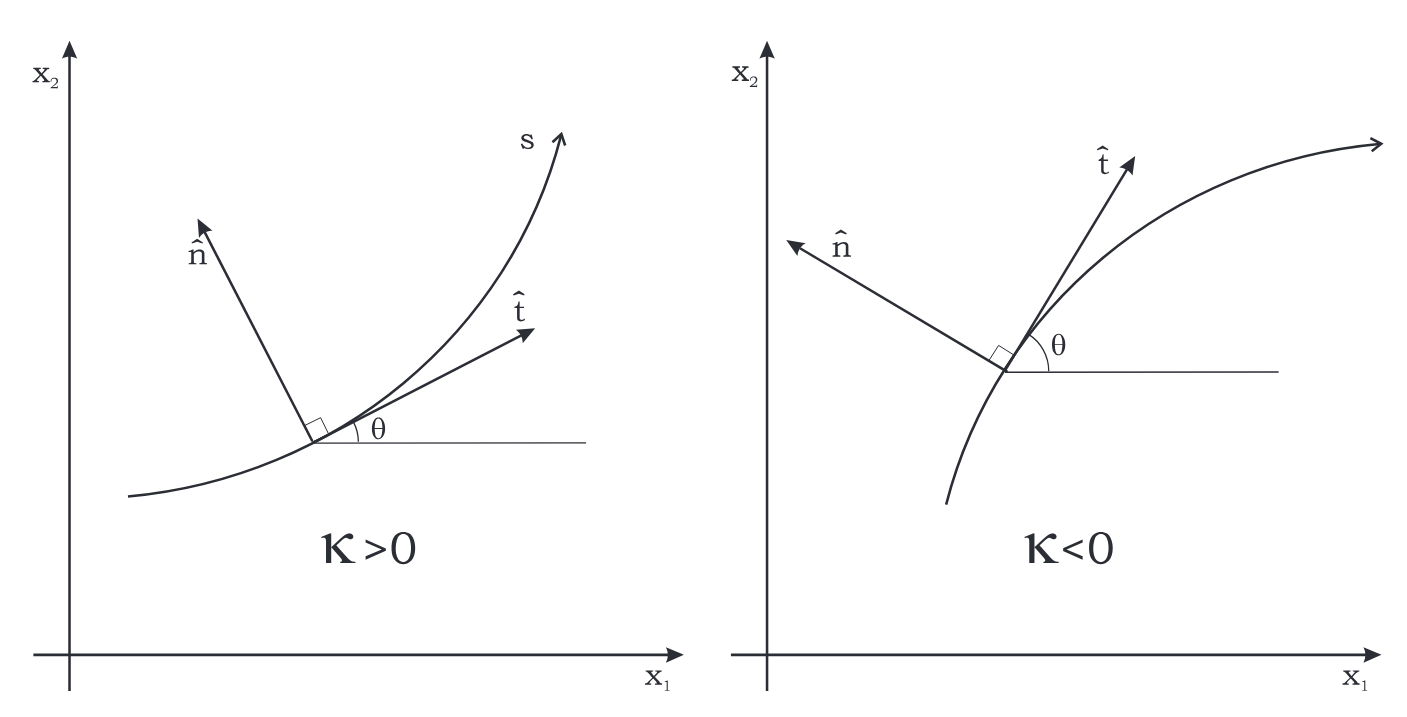
\includegraphics[width=0.95\textwidth]{assets/segno_flesso.png}
    \end{minipage}
    \caption{Segno del flesso}
\end{figure}
\vspace{-1em}
\newpage

\section{Superfici}

Più che di \emph{superfici} in senso esteso, ci interesseremo degli \emph{elementi di superficie}, poiché vogliamo esaminare le proprietà locali. Anche in questo caso, useremo una rappresentazione parametrica.

Sia
$$
\bar{x}\colon D \subseteq \mathbb{R}^2 \;\to\; \mathbb{R}^3
$$
una funzione biunivoca (dunque invertibile) che descrive una superficie nello spazio euclideo tridimensionale $E^3$. In coordinate:
$$
\bar{x}(u,v)
\;=\;
\bigl(x_1(u,v),\;x_2(u,v),\;x_3(u,v)\bigr).
$$
Se la superficie è del tipo $z = f(x,y)$, allora la parametrizzazione diventa $\bar x(u,v) = \bigl(u,\,v,\,f(u,v)\bigr)$.

\begin{figure}[H]
    \centering
    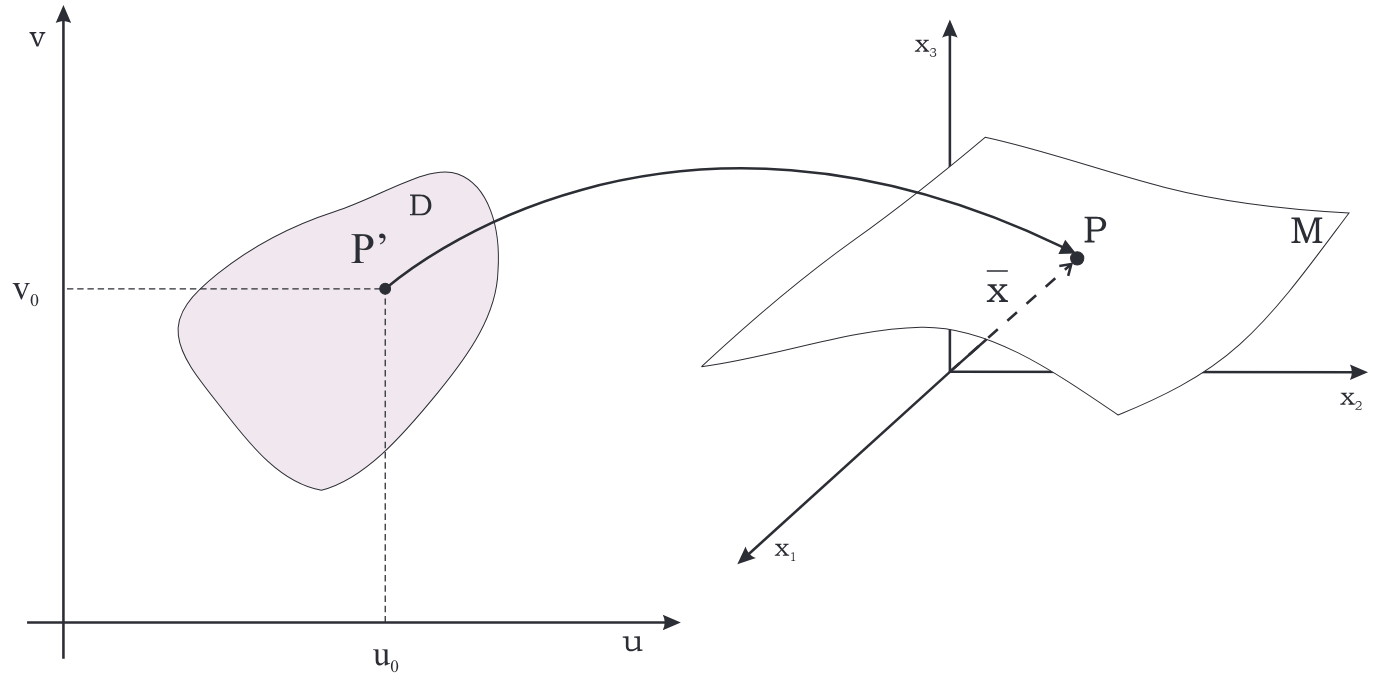
\includegraphics[width=0.7\textwidth]{assets/surface.png}
    \caption{Superficie parametrica}
\end{figure}

\begin{definitionblock}[Superficie Regolare]
Una \bfit{superficie regolare} (o \emph{smooth}) è tale se, definendo
$$
\bar{x}_u
\;=\;
\dfrac{\partial \bar{x}}{\partial u}
\;=\;
\Bigl(\dfrac{\partial x_1}{\partial u},\;\dfrac{\partial x_2}{\partial u},\;\dfrac{\partial x_3}{\partial u}\Bigr),
\qquad
\bar{x}_v
\;=\;
\dfrac{\partial \bar{x}}{\partial v}
\;=\;
\Bigl(\dfrac{\partial x_1}{\partial v},\;\dfrac{\partial x_2}{\partial v},\;\dfrac{\partial x_3}{\partial v}\Bigr),
$$
si ha che in ogni punto del dominio (cioè ovunque in $D$) risulta
$$
\bar{x}_u \;\times\; \bar{x}_v \;\neq\; 0.
$$
\end{definitionblock}

Fissando $v=v_0$ e variando $u$ nei pressi di un punto $P'\!\in D$ (che corrisponde al punto $P$ sulla superficie $M$), si ottiene una curva su $M$ il cui vettore tangente è $\bar{x}_u$. Analogamente, $\bar{x}_v$ è tangente a un’altra curva, e i due vettori definiscono il piano tangente in $P$.

Un versore normale alla superficie è dato da
\vspace{0.4em}
$$
\hat{n}
\;=\;
\dfrac{\bar{x}_u \times \bar{x}_v}{\bigl|\bar{x}_u \times \bar{x}_v\bigr|},
$$
e i tre vettori $\hat{n},\,\bar{x}_u,\,\bar{x}_v$ formano un triedro locale.

Poiché la corrispondenza tra $D$ e l’intorno di $P$ su $M$ è biunivoca, possiamo considerare $(u,v)$ come un sistema di coordinate curvilinee sull’intorno di $P$ (ad esempio, i paralleli e i meridiani su una sfera).

\newpage

Se $u=u(t)$ e $v=v(t)$ descrivono una curva in $D$ passante per $P'(u_0,v_0)$, allora
\vspace{0.4em}
$$
\bar{r}(t)
\;=\;
\bar{x}\bigl(u(t),\,v(t)\bigr)
$$

rappresenta la curva su $M$ passante per $\bar{x}(u_0,v_0)$. Il vettore velocità è

$$
\dot{\bar{r}}
\;=\;
\frac{d\bar{r}}{dt}
\;=\;
\bar{x}_u \;\frac{du}{dt}
\;+\;
\bar{x}_v \;\frac{dv}{dt}.
$$

\begin{figure}[H]
    \centering
    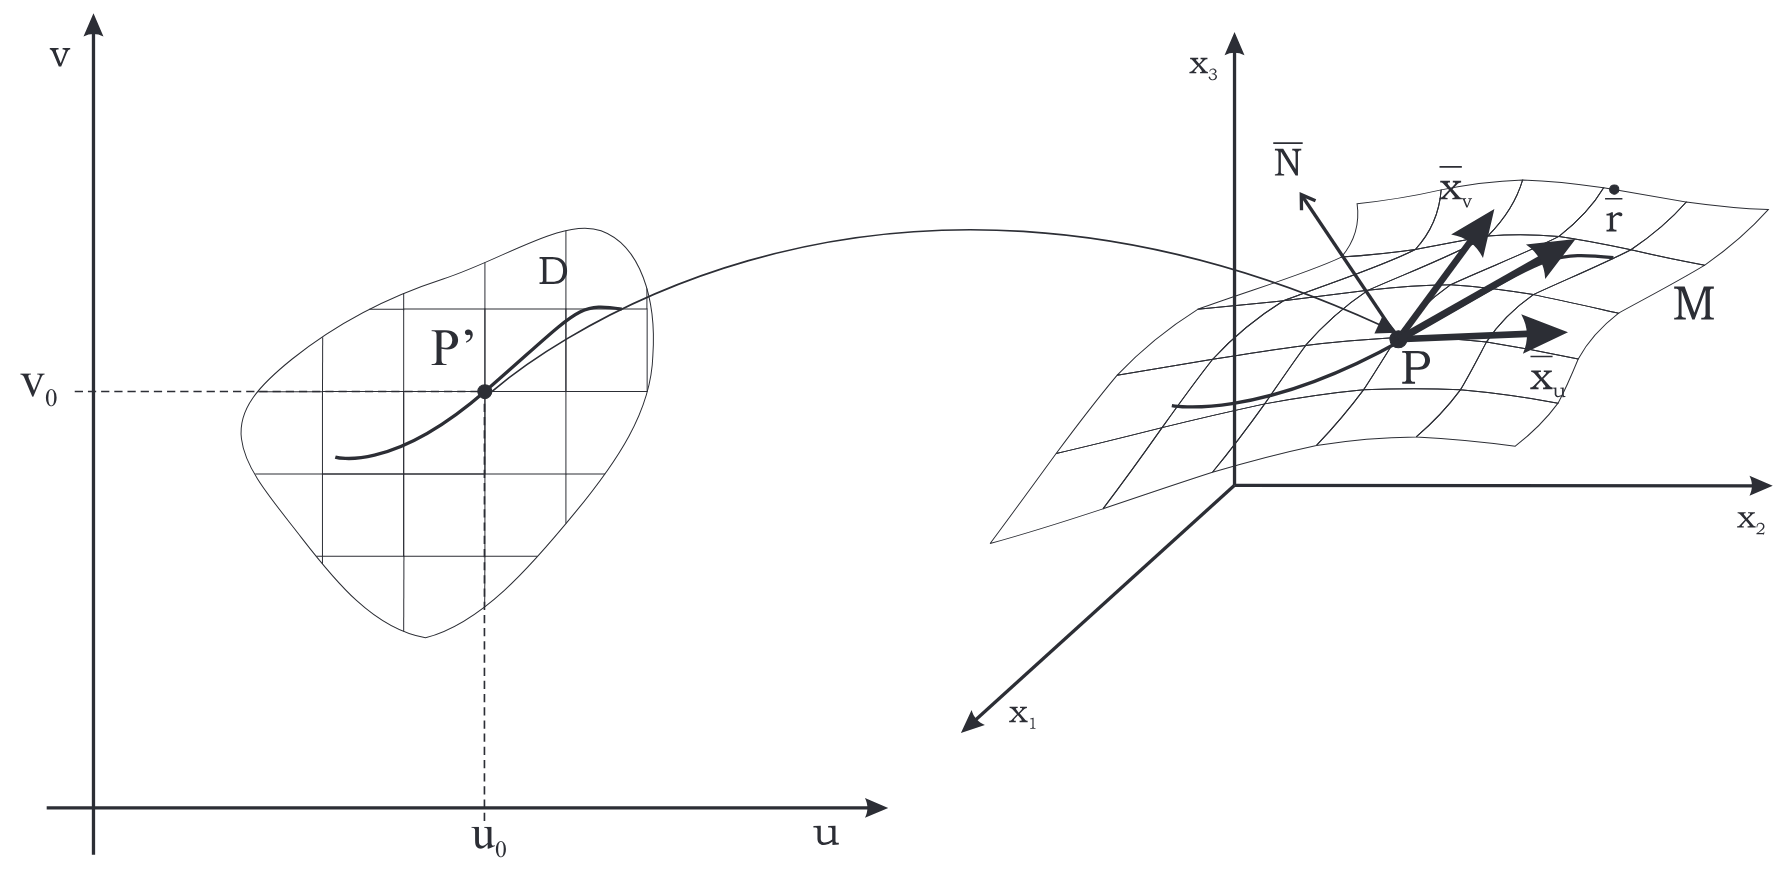
\includegraphics[width=0.7\textwidth]{assets/plane_trasf.png}
    \caption{Curva su una superficie}
\end{figure}

Poiché $\dot{\bar{r}}$ è tangente alla curva e appartiene quindi al piano tangente di $M$, ogni vettore tangente a $M$ in $P$ si può scrivere come combinazione lineare di $\bar{x}_u$ e $\bar{x}_v$. Viceversa, per ogni combinazione $\,\bar{v} = a\,\bar{x}_u + b\,\bar{x}_v\,$ esiste una corrispondente curva su $M$ la cui velocità è esattamente $\bar{v}$. In tal senso, $\bar{x}_u$ e $\bar{x}_v$ formano una base del piano tangente.

\begin{exampleblock}[Superficie di una sfera di raggio $R$]
Consideriamo la sfera di raggio $R$ centrata nell’origine. La sua superficie si parametrizza come
$$
\bar{x}(u,v)
\;=\;
\bigl(R \cos u \cos v,\;R \,\sin u \,\cos v,\;R \,\sin v\bigr),
$$
con $u \in [-\pi,\;\pi]$ e $v \in \bigl[-\tfrac{\pi}{2},\;\tfrac{\pi}{2}\bigr]$.
\vspace{0.5em}

Calcoliamo le derivate rispetto a $u$ e $v$:
\vspace{0.4em}
$$
\begin{array}{l}
\bar{x}_u
\;=\;
\dfrac{\partial \bar{x}}{\partial u}
\;=\;
\bigl(-R \sin u \cos v,\;R \cos u \cos v,\;0\bigr),
\\
\bar{x}_v
\;=\;
\dfrac{\partial \bar{x}}{\partial v}
\;=\;
\bigl(-R \cos u \sin v,\;-R \sin u \sin v,\;R \cos v\bigr).
\end{array}
$$

Consideriamo il punto $(u,v) = (0,\,0)$:
\vspace{0.4em}
$$
\bar{x}_u\bigl(0,0\bigr)
\;=\;
(0,\;R,\;0),
\qquad
\bar{x}_v\bigl(0,0\bigr)
\;=\;
(0,\;0,\;R).
$$
Tali vettori definiscono il piano tangente alla sfera in quel punto.

Il versore normale alla superficie in $(0,0)$ si ottiene con il prodotto vettoriale:
$$
\hat{n}
\;=\;
\frac{\bar{x}_u \times \bar{x}_v}{\bigl|\bar{x}_u \times \bar{x}_v\bigr|}
\;=\;
\frac{(-R^2,\,0,\,0)}{R^2}
\;=\;
(-1,\,0,\,0).
$$
\end{exampleblock}


\newpage

\section{Prima Forma Fondamentale}

In geometria differenziale, la \bfit{prima forma fondamentale} (o \textit{forma metrica}) di una superficie definisce la sua metrica intrinseca. Grazie a essa possiamo misurare lunghezze, angoli e aree \emph{rimanendo} sulla superficie, ossia senza far riferimento esplicito allo spazio tridimensionale in cui la superficie è immersa.

\begin{definitionblock}[Prima Forma Fondamentale]
    Sia $M$ una superficie regolare immersa in $\mathbb{R}^3$, e sia 
    \vspace{0.4em}
    $$
    \bar{x}\colon U\subset\mathbb{R}^2 \to \mathbb{R}^3
    $$
    una parametrizzazione locale di $M$. La \textbf{prima forma fondamentale} in un punto $p \in M$ è il bilineare simmetrico
    $$
    I_p\colon T_pM \times T_pM \to \mathbb{R},
    $$
    definito per ogni coppia di vettori tangenti $v, w \in T_pM$ (lo spazio tangente alla superficie $M$ passante per $p$) mediante
    $$
    I_p(v, w) = \langle d\bar{x}_p(v),\, d\bar{x}_p(w) \rangle,
    $$
    dove $\langle \cdot, \cdot \rangle$ indica il prodotto scalare euclideo in $\mathbb{R}^3$. In coordinate locali $(u,v)$, ponendo
    \vspace{0.4em}
    $$
    \bar{x}_u = \frac{\partial \bar{x}}{\partial u},\quad \bar{x}_v = \frac{\partial \bar{x}}{\partial v},
    $$
    l'espressione si riduce a
    $$
    ds^2 = E\,du^2 + 2F\,du\,dv + G\,dv^2,
    $$
    con
    $$
    E = \bar{x}_u \cdot \bar{x}_u,\quad F = \bar{x}_u \cdot \bar{x}_v,\quad G = \bar{x}_v \cdot \bar{x}_v.
    $$
    \end{definitionblock}
    
    \vspace{1em}

Sia $\bar{r}(t) = \bar{x}\bigl(u(t),\,v(t)\bigr)$, con $t\in[a,b]$, una curva su una superficie; se $s(t)$ è la relativa ascissa curvilinea, la lunghezza totale della curva risulta
\vspace{0.4em}
$$
L \;=\; s(b) 
\;=\; \int_a^b \frac{ds}{dt}\,dt 
\;=\; \int_a^b \bigl|\dot{\bar{r}}(t)\bigr| \,dt.
$$
Poiché
$$
\dot{\bar{r}}
\;=\;
\frac{d\bar{r}}{dt}
\;=\;
\bar{x}_u\,\dot{u}
\;+\;
\bar{x}_v\,\dot{v}
\quad\text{(dove }\dot{u} = \tfrac{du}{dt},\; \dot{v} = \tfrac{dv}{dt}\text{),}
$$
segue che
\vspace{0.4em}
$$
\biggl(\frac{ds}{dt}\biggr)^2
\;=\;
\bigl\lvert \dot{\bar{r}}\bigr\rvert^2
\;=\;
\dot{\bar{r}}\cdot \dot{\bar{r}}
\;=\;
(\bar{x}_u\,\dot{u} + \bar{x}_v\,\dot{v}) \cdot (\bar{x}_u\,\dot{u} + \bar{x}_v\,\dot{v})
\;=\;
\dot{u}^2\,(\bar{x}_u\cdot\bar{x}_u)
\;+\;
2\,\dot{u}\,\dot{v}\,(\bar{x}_u\cdot\bar{x}_v)
\;+\;
\dot{v}^2\,(\bar{x}_v\cdot\bar{x}_v).
$$

Introduciamo le funzioni
\vspace{0.4em}
$$
E \;=\; \bar{x}_u \cdot \bar{x}_u,
\quad
F \;=\; \bar{x}_u \cdot \bar{x}_v,
\quad
G \;=\; \bar{x}_v \cdot \bar{x}_v
\qquad\longrightarrow\qquad
E=E(u,v),\; F=F(u,v),\; G=G(u,v),
$$

e otteniamo
\vspace{0.4em}
$$
\biggl(\frac{ds}{dt}\biggr)^2
\;=\;
E\,\dot{u}^2
\;+\;
2\,F\,\dot{u}\,\dot{v}
\;+\;
G\,\dot{v}^2.
$$

Pertanto, la lunghezza totale della curva è
\vspace{0.4em}
$$
L
\;=\;
\int_a^b
\sqrt{\,E\,\dot{u}^2 
\;+\;
2\,F\,\dot{u}\,\dot{v}
\;+\;
G\,\dot{v}^2\,}\,dt
\;=\;
\int_{\bar{r}}
\sqrt{\,E\,du^2 \;+\; 2\,F\,du\,dv \;+\; G\,dv^2\,},
$$
che in forma differenziale si esprime come
\vspace{0.5em}
$$
\boxed{
ds^2
\;=\;
E\,du^2
\;+\;
2\,F\,du\,dv
\;+\;
G\,dv^2.
}
$$
Questa espressione, chiamata \bfit{prima forma fondamentale}, descrive la geometria intrinseca della superficie. “Intrinseco” significa che tutte le misure (di distanze, angoli, ecc.) possono essere effettuate senza “uscire” dallo spazio bidimensionale della superficie.

Poiché esiste una corrispondenza biunivoca tra $D\subset \mathbb{R}^2$ e la porzione di superficie $M$, le linee $u=\text{cost}$ e $v=\text{cost}$ formano sulla superficie una \emph{griglia} di coordinate curvilinee, mentre $E(u,v)$, $F(u,v)$ e $G(u,v)$ sono interpretate come \emph{funzioni} definite su $M$. In questo modo, ipotetici “abitanti” bidimensionali potrebbero compiere misurazioni di distanze \emph{sulla superficie} per determinare la forma di $E$, $F$ e $G$, giungendo così a una descrizione completa della metrica locale.

\begin{exampleblock}[Il piano]
Consideriamo il piano in $E^3$ descritto da $\bar{x}(u,v)=(u,\,v,\,0)$, con coordinate cartesiane $x=u$ e $y=v$. Allora
$$
\bar{x}_u=(1,0,0), 
\quad
\bar{x}_v=(0,1,0),
$$
e i coefficienti della prima forma fondamentale sono
$$
E=\bar{x}_u\cdot\bar{x}_u=1,\quad
F=\bar{x}_u\cdot\bar{x}_v=0,\quad
G=\bar{x}_v\cdot\bar{x}_v=1.
$$
Quindi,
$$
ds^2=du^2+dv^2,
$$
che corrisponde al classico \emph{teorema di Pitagora} in forma differenziale. La lunghezza di una curva $y=f(x)$, parametrizzata da $x=t$ e $y=f(t)$, è
$$
L
\;=\;
\int_a^b \sqrt{1 + \bigl(f'(x)\bigr)^2}\,dx.
$$
\end{exampleblock}

\begin{exampleblock}[Sfera in coordinate sferiche]

    Consideriamo una sfera di raggio $R$ centrata nell'origine. La superficie della sfera è data da:
    
    \small
    $$
    \bar x(u,v) = (R \cos u \cos v, R \sin u \cos v, R \sin v)
    \ \ \xrightarrow{\text{derive}} \ \
    \begin{cases}
        \bar x_u = (-R \sin u \cos v, R \cos u \cos v, 0)
        \\
        \bar x_v = (-R \cos u \sin v, -R \sin u \sin v, R \cos v)
    \end{cases}
    $$
    \normalsize
    
    dove $u \in [-\pi, \pi]$, $v \in [-\pi/2, \pi/2]$
    
    Calcoliamo i coefficienti della prima forma fondamentale:
    
    $$
    \begin{cases}
    E = \bar{x}_u \cdot \bar{x}_u = R^2 \cos^2 v \sin^2 u + R^2 \cos^2 v \cos^2 u & = R^2 \cos^2 v
    \\
    G = \bar{x}_v \cdot \bar{x}_v = R^2 \sin^2 v \cos^2 u + R^2 \sin^2 v \sin^2 u + R^2 cos^2 v & = R^2 
    \\
    F = \bar{x}_u \cdot \bar{x}_v = R^2 v \cos v \cos u \sin \sin u - R^2 \cos v \cos u \sin \sin u & = 0
    \end{cases}
    $$
    
    Quindi, la prima forma fondamentale è:
    
    $$
    ds^2 = R^2 \cos^2 v\, du^2 + R^2 dv^2
    $$
    
\end{exampleblock}

\subsection{Identità di Lagrange}

L'identità di Lagrange è una relazione che lega la forma metrica e la prima forma fondamentale di una superficie.

Se
$
\begin{cases}
    \bar v = a\bar x_u + b\bar x_v \\ 
    \bar \omega = c\bar x_u + d\bar x_v
\end{cases}
\text{, con } a,b,c,d \in \mathbb{R}
$
, sono due vettori tangenti alla superficie $M$, allora:

$$
\bar v \cdot \bar \omega = (a\bar x_u + b\bar x_v) \cdot (c\bar x_u + d\bar x_v) = acE + (ad + bc)F + bdG
$$

che si può riscrivere nella forma matriciale:

$$
\begin{pmatrix}
    a & b \\
\end{pmatrix}
\underbrace{
\begin{pmatrix}
E & F \\
F & G
\end{pmatrix}
}_{\text{\scriptsize Forma metrica}}
\begin{pmatrix}
    c \\
    d
\end{pmatrix}
$$

nella quale la compare la matrice della prima forma fondamentale (forma metrica).

Quindi la conoscenza della prima forma fondamentale permette di calcolare prodotti scalari su $M$, e quindi non
solo lunghezze ma anche angoli.

Ricordiamo che, essendo $\bar x_u \times \bar x_v$ perpendicolare al piano tangente alla superficie, il versore normale $\hat N =  \dfrac{\bar x_u \times \bar x_v}{|\bar x_u \times \bar x_v|}$ è perpendicolare alla superficie.

\vspace{1em}

\renewcommand{\qedsymbol}{C.V.D.}

\newtheorem{theorem}{Teorema}[chapter]
\begin{theorem}

    \textbf{Identità di Lagrange}

    La quantità $|\bar x_u \times \bar x_v|^2$ è uguale al determinante della matrice della prima forma fondamentale:
    $$
    |\bar x_u \times \bar x_v|^2 =
    \det
    \begin{pmatrix}
        E & F \\
        F & G
    \end{pmatrix}
    $$
\end{theorem}
\begin{proof}[\textbf{Dimostrazione}:]
    \phantom{}

    Ricodiamo che: $
    \quad
    \left\{
    \begin{array}{ccl}
    |\bar x_u \times \bar x_v| & = & |\bar x_u| |\bar x_v| \sin \theta
    \\
    \bar x_u \cdot \bar x_v & = & |\bar x_u| |\bar x_v| \cos \theta
    \end{array}
    \right.
    \quad
    $
    dove $\theta$ è l'angolo tra $\bar x_u$ e $\bar x_v$.
    
    Elevando al quadrato, otteniamo:

    $$
    |\bar x_u \times \bar x_v|^2 = (|\bar x_u|^2 |\bar x_v|^2 \sin^2 \theta) = |\bar x_u|^2 |\bar x_v|^2 (1 - \cos^2 \theta) = \underbrace{|\bar x_u|^2}_E \cdot \underbrace{|\bar x_v|^2}_G - \underbrace{(\bar x_u \cdot \bar x_v)^2}_{F^2}
    $$

    
    Ricordando che $|\bar x_u \times \bar x_v|^2 = \det \begin{pmatrix} E & F \\ F & G \end{pmatrix}$, otteniamo l'identità di Lagrange:
    
    $$
    \det \begin{pmatrix} E & F \\ F & G \end{pmatrix} = EG - F^2
    $$ 
\end{proof}

Dalla condizione che la superficie sia regolare, segue che $E G - F^2 \neq 0$

\vspace{1em}

A questo punto facciamo un cambiamento nella simbologia usata; come vedremo questo porterà ad una notevole semplificazione delle formule.

Chiamiamo: $\quad
g_{11} \equiv E, \quad g_{12} = g_{21} \equiv F, \quad g_{22} \equiv g, \qquad \bar x_1 \equiv \bar x_u, \quad \bar x_2 \equiv \bar x_v
$

E scriviamo $\quad u^1 \equiv u, \quad u^2 = v \quad$ (dove gli apici 1 e 2 sono indici alti e non esponenti).9

Allora avremo $g_{ij} = \bar x_i \cdot \bar x_j \ \ (i,j = 1,2)$ e la matrice della forma metrica sarà:

$$
\begin{pmatrix} g_{11} & g_{12} \\ g_{21} & g_{22} \end{pmatrix} = \begin{pmatrix} E & F \\ F & G \end{pmatrix}
$$

Ricordiamo che $g_{ij} = g_{ij}(u, v) = g_{ij}(u^1, u^2)$

detto $g = det(g_{ij}) = EG - F^2$, allora (dall'identità di Lagrange) $|\bar x_1 \times \bar x_2|^2 = g$.

Nella nuova notazione la prima forma fondamentale diventa:

$$
ds^2 = g_{11} (du^1)^2 + 2g_{12} du^1 du^2 + g_{22} (du^2)^2 = g_{ij} du^i du^j
$$

\begin{tipsblock}[Notazione di Einstein]
Nella \emph{notazione di Einstein}, quando un indice compare una volta in alto e una in basso, si sottointende una somma su tutti i valori possibili di tale indice. Per esempio, $g_{ij}\,du^i\,du^j$ significa $\sum_{i,j} g_{ij}\,du^i\,du^j$.
\end{tipsblock}

Abbiamo usato la relazione $2g_{12} = g_{12} + g_{21}$ poiché la forma metrica è simmetrica, ossia $g_{ij} = g_{ji}$.

Un vettore tangente alla superficie $M$ nel punto $P$ può essere scritto come
$$
\bar v = a\,\bar x_1 + b\,\bar x_2,
$$
oppure, in forma esplicita,
$$
\bar v = v^1\,\bar x_1 + v^2\,\bar x_2 = \sum_{i} v^i\,\bar x_i,
$$
dove l'indice $i$ è una variabile indicizzata (è intercambiabile con altre lettere).

Se consideriamo due vettori tangenti $\bar v = \sum_{i} v^i\,\bar x_i$ e $\bar w = \sum_{j} w^j\,\bar x_j$, entrambi definiti in $P$, il loro prodotto scalare risulta:
$$
\bar v \cdot \bar w 
=\; \sum_{i,j} \Bigl( v^i\,\bar x_i \cdot w^j\,\bar x_j \Bigr)
=\; \sum_{i,j} v^i\,w^j\,(\bar x_i \cdot \bar x_j)
=\; \sum_{i,j} g_{ij}\,v^i\,w^j.
$$
I vettori $\bar v$ e $\bar w$ sono ortogonali se e solo se $\sum_{i,j} g_{ij}\,v^i\,w^j = 0$

Definiamo ora $g^{ij}$ come gli elementi della matrice inversa di $g_{ij}$, in modo tale che:
\vspace{0.4em}
$$
\begin{pmatrix}
    g_{11} & g_{12} \\
    g_{21} & g_{22}
\end{pmatrix}
\begin{pmatrix}
    g^{11} & g^{12} \\
    g^{21} & g^{22}
\end{pmatrix}
=
\begin{pmatrix}
    1 & 0 \\
    0 & 1
\end{pmatrix},
$$
ovvero, in forma compatta,
$$
\sum_{j} g_{ij}\,g^{jk} = \delta_i^k,
$$
dove $\delta_i^k$ è la \bfit{delta di Kronecker} (matrice identità), definita da: 
$
\quad
\delta_i^k =
\begin{cases}
    1, & \text{se } i = k, \\
    0, & \text{se } i \neq k.
\end{cases}
$

Utilizzando la formula per l'inversa di una matrice $2\times2$, otteniamo:
\vspace{0.4em}
$$
g^{11} = \dfrac{g_{22}}{g},\quad g^{12} = g^{21} = -\dfrac{g_{12}}{g},\quad g^{22} = \dfrac{g_{11}}{g},
$$
dove $g = \det(g_{ij}) = g_{11}\,g_{22} - g_{12}^2$.

Osserviamo ora come la prima forma fondamentale consenta non solo di determinare distanze e angoli, ma anche di calcolare le aree.

Sia $x: D \to E^3$ una superficie e sia $\Omega\subset D$ una regione del dominio in cui $x$ è biunivoca. Per calcolare l'area di $x(\Omega)$ suddividiamo $\Omega$ in piccoli rettangoli, tracciando linee parallele agli assi delle coordinate $u^1$ e $u^2$.

\begin{figure}[H]
    \centering
    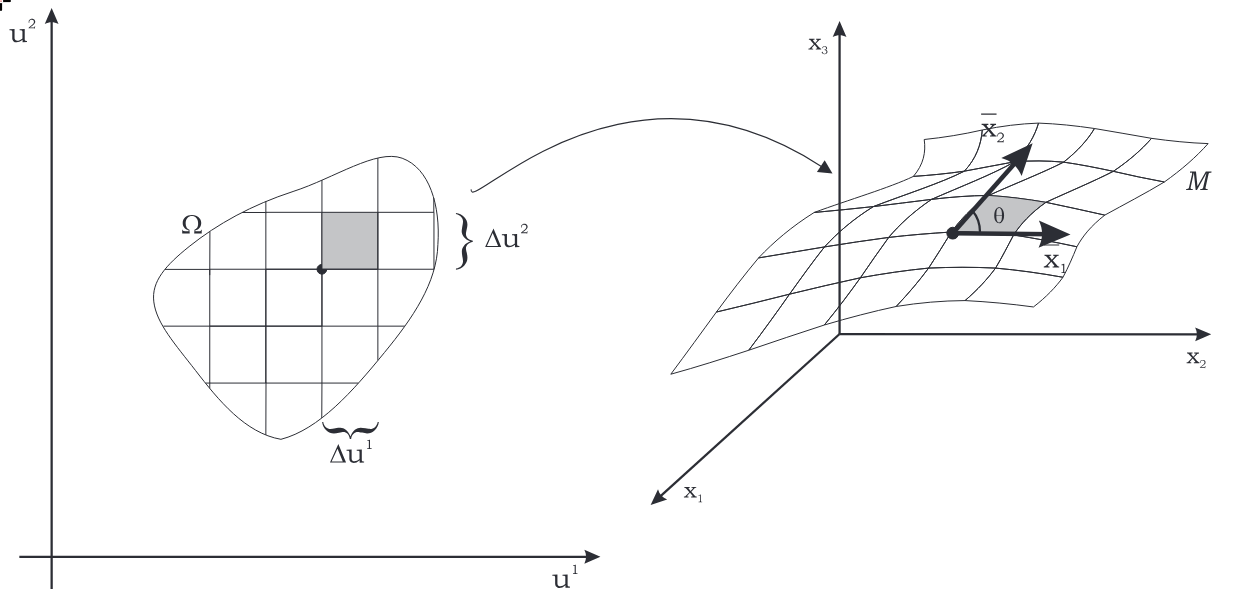
\includegraphics[width=0.75\textwidth]{assets/area.png}
    \caption{Area di una superficie}
\end{figure}

Ad una piccola areola di $\Omega$ con lati $\Delta u^1$ e $\Delta u^2$ corrisponde, approssimativamente, un pezzo di superficie a forma di parallelogramma, i cui lati sono paralleli ai vettori $\bar x_1$ e $\bar x_2$. Le lunghezze dei lati sono rispettivamente
$$
\Delta l_1 \simeq |\bar x_1|\,\Delta u^1,\qquad \Delta l_2 \simeq |\bar x_2|\,\Delta u^2.
$$
Ricordiamo che, per definizione, $|\bar x_1| = \left|\frac{\partial \bar x}{\partial u^1}\right|$, per cui
\vspace{0.4em}
$$
\Delta \bar x_1 = \frac{\partial \bar x}{\partial u^1}\,\Delta u^1.
$$
L'area dell'areola è data da
\vspace{0.4em}
$$
\Delta A = |\bar x_1|\,\Delta u^1 \cdot |\bar x_2|\,\Delta u^2\,\sin\theta 
=\; |\bar x_1 \times \bar x_2|\,\Delta u^1\,\Delta u^2
=\; \sqrt{g}\,\Delta u^1\,\Delta u^2,
$$
dove $\theta$ è l'angolo tra $\bar x_1$ e $\bar x_2$ e $g = \det(g_{ij})$.

Passando al limite in cui $\Delta u^1,\,\Delta u^2 \to 0$ e sommando su tutte le areole, l'area di $x(\Omega)$ è data da:
\vspace{0.4em}
$$
A = \iint_{\Omega} \sqrt{g}\,du^1\,du^2.
$$

Osserviamo che, in due dimensioni, la misura di un insieme coincide con l'area; in spazi di dimensione $n$, l'integrale di $\sqrt{g}$ fornisce rispettivamente un volume $n$-dimensionale. Questo procedimento vale per spazi (o \emph{manifolds}) \bfit{Riemanniani}, in cui $ds^2>0$. Negli spazi \bfit{pseudo-Riemanniani} (ad esempio, lo \emph{spazio-tempo di Minkowski} nella Relatività Speciale) alcuni elementi del tensore metrico possono essere negativi; in tali casi, poiché il determinante $g$ può risultare negativo, si usa in generale $\sqrt{|g|}$.

\begin{exampleblock}[Sfera]
    La sfera è uno spazio Riemanniano:
    $$
    ds^2 = R^2 \cos^2 v du^2 + R^2 dv^2
    \qquad
    \begin{cases}
    - \pi < u < \pi \\
    - \frac{\pi}{2} < v < \frac{\pi}{2}
    \end{cases}
    $$
    Otteniamo la matrice:
    $$
    g_{ij} = \begin{pmatrix}
        R^2 \cos^2 v & 0 \\
        0 & R^2
    \end{pmatrix}
    \quad \Rightarrow \quad
    g = R^4 \cos^2 v, \quad \sqrt{g} = R^2 \cos v
    $$
    Calcoliamo l'area:
    $$
    A = \iint_{\Omega} \sqrt{g} du dv = \int_{-\pi}^{\pi} du \int_{-\frac{\pi}{2}}^{\frac{\pi}{2}} R^2 \cos v dv = \boxed{4 \pi R^2}
    $$
\end{exampleblock}

\begin{exampleblock}[Toro]
    Consideriamo un esmepio più complesso, il toro:

    $$
    \bar x (u, v) = [R + r \cos u] \cos v, [R + r \cos v] \sin u, r \sin v,
    $$
    
    \begin{minipage}[H]{0.5\textwidth}
        $$
        \begin{cases}
            0 < v < 2\pi \\
            0 < u < 2\pi \\
            0 < r < r
        \end{cases}
        $$
    \end{minipage}%
    \begin{minipage}[H]{0.5\textwidth}
        \begin{figure}[H]
            \centering
            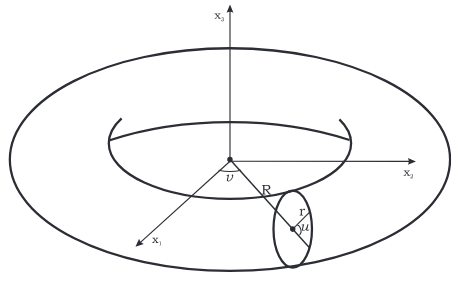
\includegraphics[width=0.6\textwidth]{assets/toro.png}
        \end{figure}
    \end{minipage}
    
    Otteniamo:

    $$
    A = \iint_{\Omega} \sqrt{g} du dv = \boxed{4 \pi^2 R r}
    $$

\end{exampleblock}